\subsection{Overview}

\subsection{Component view}
In order to give a better description of the component of the system, the below class diagram shows how the application is designed.

All this description regards only the application tier of the system. This portion communicate to the client via the web server.

 The communication between the web server and the application is made by an interface exposed to the web server (SystemMangerInterface).
 
The client, used by users and authority that want to see statistics, does not contain any portion of the logic of the system (except for the GPS rilevation). Thus it is a thin client and no class diagram has been made for it.

In the note of the diagram it is possible to see which design patterns has been implemented (facade and singleton).

The data are stored in the database (data tier) are accessible using the mananger classes. Their function is to query the database and save the data retrived in the appropriate object (for every entity of the database a spefic class has been designed).

All the request arriving from clients are catched by the web server. Then it calls the appropriate method of facade class SystemMananger using the interface SystemMangerInterface. This class uses the method of the other to respond to the request.

Periodically the SystemManager method for obtaing information on accidents occured, is called. It retrieves the information and then stores then in the database.

During the registration process of an authority the specific method calls a web service to check the authenticity of the CUU code.

Moreover, an interface is exposed to authoties system. In this way the can call a method that provide the reports data and generate traffic tickets on them. Before sending any type of information the identity of the authority is checked using the appropriate method of UserManager class.

\begin{figure}[H]
	\centering
	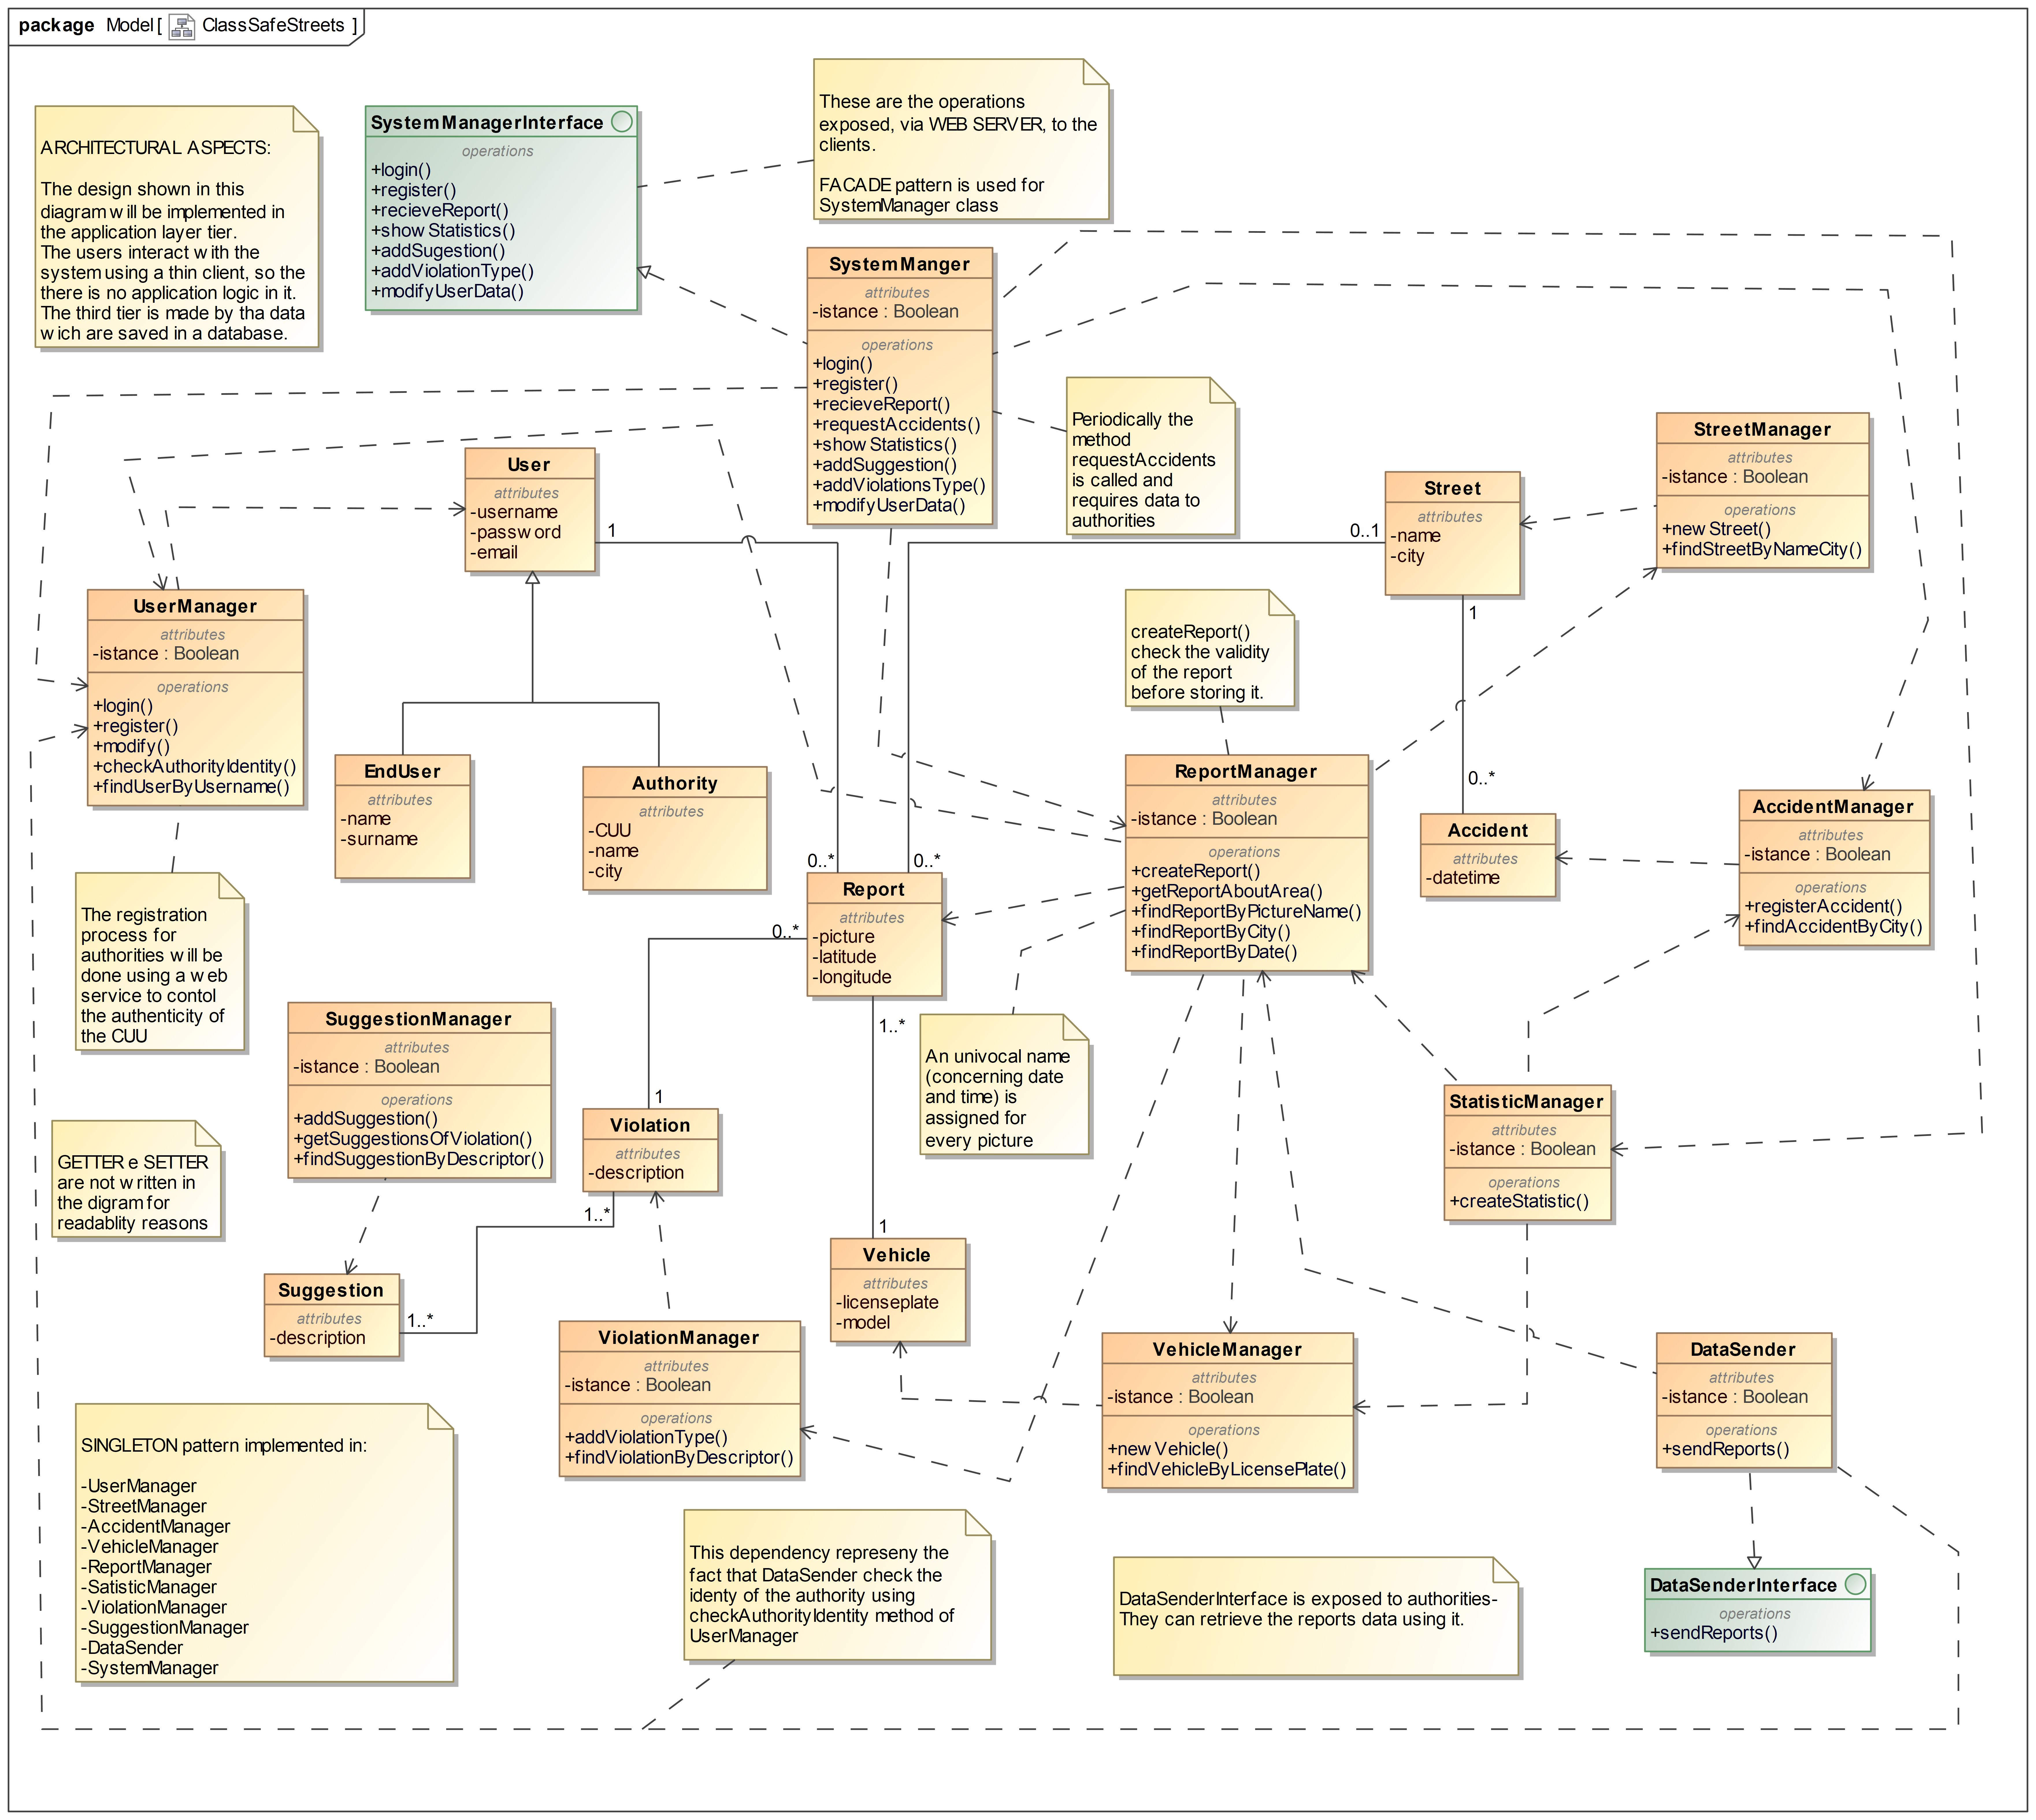
\includegraphics[width=1.12\linewidth]{Images/ClassSafeStreets.png}
	\caption{Class diagram}
\end{figure}

The component diagram below describes the implementation of the classes described before in terms of components.

The macro-component SafeStretsApplication represents the application running on the application server. It exposes two interface. The first one is designed to communicate with the web server that catch the clients requests. The second is exposed to authority systems in order to offer information that can be used to generate traffic tickets.

There are also subcomponents that perform specific operations and interact with the database:
\begin{itemize}
 \item 
 SystemManager: is the component that conveys all the request to the appropriate subcomponents and periodically activate the AccidentManager.
 \item 
 AccidentManager: is the component that calls the specific service to retrieve the data about accidents occured. These informations will be used by StatisticManager.
 \item
 StatisticManager: is the component designed to create statistic crossing data coming from report and accidents.
 \item 
 PositionManager: is the component used to organize data about position and streets.
 \item 
 UserManager: is the component used to manage user operations (for istance login,registration...).
 \item
 ReportSender: it is used to send data about reports stored to authority system. These information will be used to generate traffic tickets. This subcomponent exposes directly an interface to the external enviroment. Naturally before sending the data, the method check the identity of the authority using the UserManager.
 \item 
 VehicleManger: is the component designed to manage the data about vehicle.
 \item 
 ViolationAndSuggestionMangaer: it is used to store and modify the type of violation and suggestion.
 \item 
 ReportMangaer: is the component that store reports in the database and retrive information on it.
 
\end{itemize}

\begin{figure}[H]
	\centering
	\includegraphics[width=1.12\linewidth]{Images/component.png}
	\caption{Component diagram}
\end{figure}

\subsection{Deployment view}
In the deployment diagram below it is possible to see the physical implementation of the system.
SafeStreets is composed by 3 nodes:
\begin{itemize}
	\item 
	First tier: represent the thin clien that make HTTP requests. It is used by users for sending reports and by authorities in order to see statistics.
	\item 
	Second tier: is made by the web server and the appliaction server. The first one is responsible of the catching of the HTTP requests coming from the clients. The web server read the requests and call the appropriate method exposed by the application server. The real computation of the requests is done here.
	When data stored are required, the application server communicates with the third tier.
	\item 
	Second tier: this tier represent the database of the system. 
\end{itemize} 

In the diagram there is also an other node that corresponds with the authority system in charge of retrieving reports to generate traffic tickets. The application server exposes a interface that provides this function. 

\begin{figure}[H]
	\centering
	\includegraphics[width=1.12\linewidth]{Images/Deployment.png}
	\caption{Deployment diagram}
\end{figure}
